\begin{center}
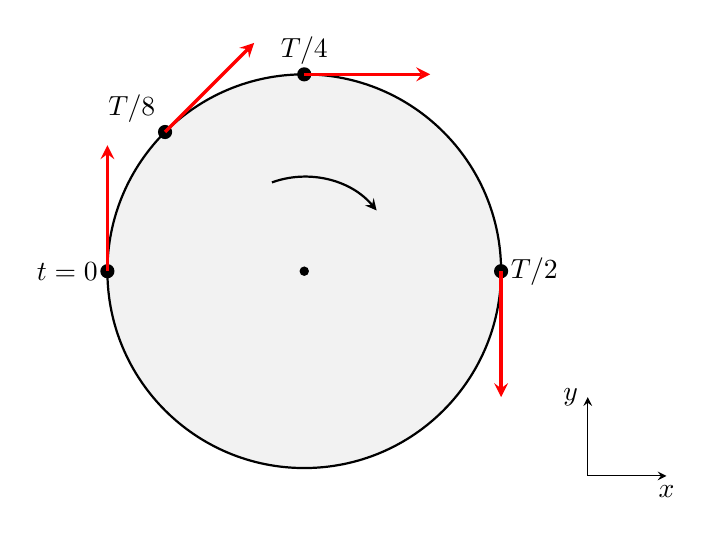
\begin{tikzpicture}[>=stealth]
 \draw[thick, fill=gray!10] (0,0) circle (2.5);
 \fill (0,0) circle (0.06);
 \draw[->, thick] (110:1.2) arc (110:40:1.2);
 \fill (180:2.5) circle (0.09) node[left] {$t=0$};
 \draw[->, very thick, red] (180:2.5) -- ++(90:1.6);
 \fill (135:2.5) circle (0.09) node[above left] {$T/8$};
 \draw[->, very thick, red] (135:2.5) -- ++(45:1.6);
 \fill (90:2.5) circle (0.09) node[above] {$T/4$};
 \draw[->, very thick, red] (90:2.5) -- ++(0:1.6);
 \fill (0:2.5) circle (0.09) node[right] {$T/2$};
 \draw[->, very thick, red] (0:2.5) -- ++(-90:1.6);
 \draw[->] (3.6,-2.6) -- (4.6,-2.6) node[below] {$x$};
 \draw[->] (3.6,-2.6) -- (3.6,-1.6) node[left] {$y$};
\end{tikzpicture}
\end{center}

Der Geschwindigkeitsvektor steht immer senkrecht zum Radius und dreht sich deshalb mit dem Punkt mit: In der Zeit $t$ dreht er sich um den Winkel $\varphi = 2\pi\,t/T$ im Uhrzeigersinn, sein Betrag $v = \vsO$ bleibt gleich. Ein Vektor $\left(0\,\middle|\,v\right)$, der um $\varphi$ im Uhrzeigersinn gedreht wird, wird zu
\begin{align}
 \vec v(t) &= \left(v\sin\varphi\,\middle|\,v\cos\varphi\right)
\end{align}

\begin{itemize}
\item $t = T/8$, $\varphi = \ang{45}$: $v_x = v_y = \vqF = \vq$, also
\begin{align}
 \vec v &= \result{\left(\vqP{0}{2}\,\middle|\,\vqP{0}{2}\right)}
\end{align}
\item $t = T/4$, $\varphi = \ang{90}$: $\vec v = \result{\left(\vsrP{0}{2}\,\middle|\,0\right)}$
\item $t = T/2$, $\varphi = \ang{180}$: $\vec v = \result{\left(0\,\middle|\,\vsnP{0}{2}\right)}$
\end{itemize}
